\documentclass[a4paper,12pt,oneside]{article}

\usepackage[a4paper,top=3cm,bottom=3cm,left=3cm,right=3cm]{geometry}
\renewcommand{\familydefault}{\sfdefault}
\usepackage{helvet}
\usepackage[pdftex]{graphicx}
\usepackage[pdftex]{hyperref}	
\usepackage{multicol}
\usepackage[cm]{fullpage}
\usepackage{url}
\usepackage{float}
\usepackage{gensymb}
\usepackage{enumerate}
\pdfadjustspacing=1	

\setlength{\columnsep}{0.6cm}

\pagenumbering{arabic}

\newcommand{\myname}{Nikoloz Kapanadze}
\newcommand{\mytitle}{Real Time Binaural Audio Spatialization Using MAX/MSP}
\newcommand{\mysupervisor}{Prof.~M.~Bode}

\hypersetup{
  pdfauthor = {\myname},
  pdftitle = {\mytitle},
  pdfkeywords = {},
  colorlinks = {true},
  linkcolor = {blue}
}

\begin{document}
  \thispagestyle{empty}
  \begin{flushright}
    
\includegraphics[scale=0.7]{bsc-logo}
  \end{flushright}
  \vspace{20mm}
  \begin{center}
    \huge
    \textbf{\mytitle}
  \end{center}
  \vspace*{4mm}
  \begin{center}
   \Large by
  \end{center}
  \vspace*{4mm}
  \begin{center}
    \Large
    \textbf{\myname}
  \end{center}
  \vspace*{20mm}
  \begin{center}
    \large
    Bachelor Thesis Proposal in Electrical and Computer Engineering
  \end{center}
  \vfill
  \begin{flushright}
    \large
    \begin{tabular}{l}
      \mysupervisor \\
      \hline
      Name and title of the supervisor \\
      \\
    \end{tabular}
  \end{flushright}
  \vspace*{8mm}
\begin{flushleft}
\large
Date of Submission: May 10, 2015 \\
\rule{\textwidth}{1pt}
\end{flushleft}
\begin{center}
\Large Jacobs University --- School of Engineering and Science
\end{center}
\newpage
\thispagestyle{empty}

  With my signature, I certify that this thesis has been written by me
  using only the indicates resources and materials. Where I have
  presented data and results, the data and results are complete,
  genuine, and have been obtained by me unless otherwise acknowledged;
  where my results derive from computer programs, these computer
  programs have been written by me unless otherwise acknowledged. I
  further confirm that this thesis has not been submitted, either in
  part or as a whole, for any other academic degree at this or another
  institution.

\vspace{20mm}

Signature \hfill Place, Date

\newpage  
\section*{Abstract}
  
Hearing is one of the senses we use to perceive our surroundings. However the systems used nowadays to playback sound, be it music, audio effects in video games, or anything else do not take full advantage of capabilities that our ears possess. While humans are well equipped to discern the direction from which a particular sound is coming, conventional magnitude based panning methods do not relay enough cues for accurate sound localization. This paper will discuss a system that is capable of tracking the orientation of the user's head and processing of incoming audio  orientation into account using a technique called binaural spatialization taking the orientation information into account. This technique allows us to simulate directionality of sound with a finer degree of localization than other panning methods.  A system like this could have a lot of potential uses:
\begin{itemize}
\item Coupled with a VR display system it would introduce a higher level of immersion to users.
\item It has a potential to improve long distance communications experience, increasing immersion where telepresence is involved. 
\item Equipped with additional sensors that keep track of the surroundings, it could serve as an aid for people with visual impairments, as it has a way of relaying the positions of objects by means of introducing auditory cues that can be decoded into location information.
\item If used in conjunction with sampled impulse response of a specific real environment, composers or acousticians could use this system to adapt their music or equipment to particular environments remotely.
\end{itemize}

\newpage
  \tableofcontents


\section{Introduction}
\subsection{Motivation}

The motivation behind this project is to augment the listening experience by adding dimensionalty to the sound by a specific means of processing that introduces auditory cues that we humans can interpret as directional information. Most of the solutions to the spatialization problem can be divided into two categories. a) Magnitude based panning, which is more about balance of sound rather than realistic reproduction. b) Post-processing techniques that produce high fidelity result but are static in nature. The idea of this project is to turn the spatialization process into dynamic and interactive one.

\subsection{Research Question}


Based on the problems and requirements listed in the section above, the research question can be formulated as follows:\\
\textbf{Can a real-time binaural spatialization system be implemented reliably?}\\
Since this system aims to improve the listening experience, a high fidelity output with as little auditory distortions as possible is required.\\
The result of this project will be a device that is capable of performing the tasks mentioned in the sections above

\section{State of the Art}
Modern audio industry has seen many advances and improvements in recent years. Improvements in the quality of digital technologies brought the experience of listening to new heights. A lot has been done where low distortion audio acquisition and playback is concerned. Higher sampling rates and increased bit depth have made it possible to significantly increase SNR (signal to noise ratio) and reduce THD (total harmonic distortion) of audio systems. There is however one field that has seen little change for the past years, namely headphones. Arguably not much has changed about the way people listen to audio through headphones since John C. Koss of Koss Corporation first created stereo headphones in 1958. There have obviously been changes to his designs that brought various improvements, But the model audio playback systems in combination with headphones use as the de facto standard is flawed; How humans hear sounds coming from external sources, even speakers for that matter, is quite different from headphones. A lot of variables are not accounted for when distributing sound between the two audio channels. Binaural spatialization techniques allow us to model the listener as a system that has certain properties associated with it while providing us with tools needed to make the sound more realistic.\\

Binaural spatialization has been around for quite a while now. In fact, as early as in 1881 we come across Theatrophone - a binaural telephonic distribution system that used an array of microphones to record and transmit performances to customers equipped via telephone. The listeners had to be equipped with a special pair of transducers to listen to the transmissions.\\

A lot of research has been done in the field since then. One project that needs to be mentioned in this context is the CIPIC HRTF Database. This is a public-domain database of high-spatial-resolution HRTF (head related transfer function) measurements for 45 different subjects, including the KEMAR mannequin with both small and large pinnae. these measurements will be referred to a lot since they will provide the basis for modeling the listener's head during processing.\cite{cipic1}\\

It should also be noted that several audio synthesis and processing software solutions have binaural spatialization built into them or available as third party plug-ins. A notable example would be Apple's Logic Pro - a professional DAW (digital audio workstation) comes with a built in binaural panner that allows the user to specify the virtual location of sound sources in 3D. However most solutions, use this technique as a part of post processing. This means that even though the user can hard-code any dynamic changes into the location of sources, such panners do are not interactive. The position of audio sources is tied to a reference frame with its origin fixed to the position of the listener's head. This project aims to put the both the listener and the sound sources into the same static reference frame which the listener would be able to navigate through in real time.\cite{aap1}
  
\section{Theoretical Foundations}
  
\subsection{Binaural Recording}
  
Binaural recordings are a special type of recordings intended for reproduction through headphones that allow the listener to experience a realistic virtual sound scene. They create the illusion of sound sources being located in space outside the listener's head. This effect is achieved through a specific setup used for capture of sound. Microphones are placed in a dummy head's or actual person's ear canals(fig \ref{fig:binrec})to capture the sound with all the delays, reverberations and filtering that are present in the signals that ears capture in real environments. All these effects are introduced by the location of audio sources, scattering and reflections caused by various objects (the listener included) positioned in the environment.\cite{hrtf1}\\

\begin{center}
\begin{figure}[H]
    \centering
    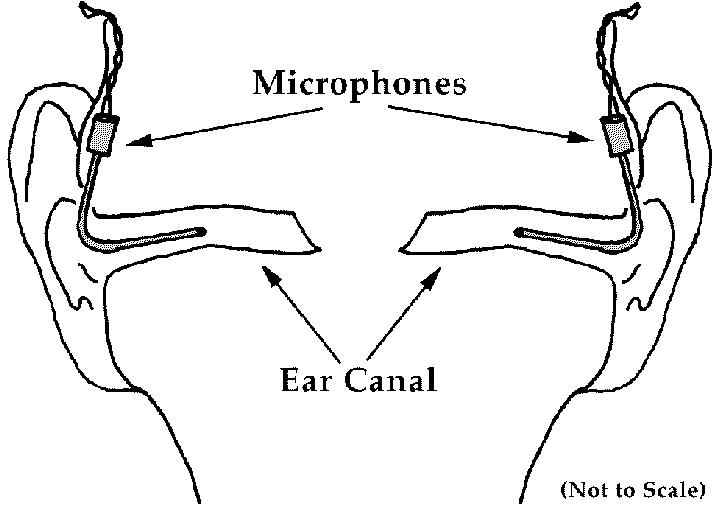
\includegraphics[scale=0.3]{binrec.jpg}
    \caption{Placement of microphones for binaural recording}
    \label{fig:binrec}
\end{figure}
\end{center}

If such a recording is played back (through headphones) to a person whose head and ear shape matches or is similar to the model used during the recording process, the brain of this person should be able to externalize the sound (perceive it as coming from outside the head) and decode the auditory cues such as IDT (Interaural Delay Time - the difference between the times it takes the sound to reach the left and right ears) and reconstruct the sound scene based on that.(fig \ref{fig:idt}) There is a way of achieving the same effect without the hassle of going through the complicated recording process every time.\\

\begin{center}
\begin{figure}[H]
    \centering
    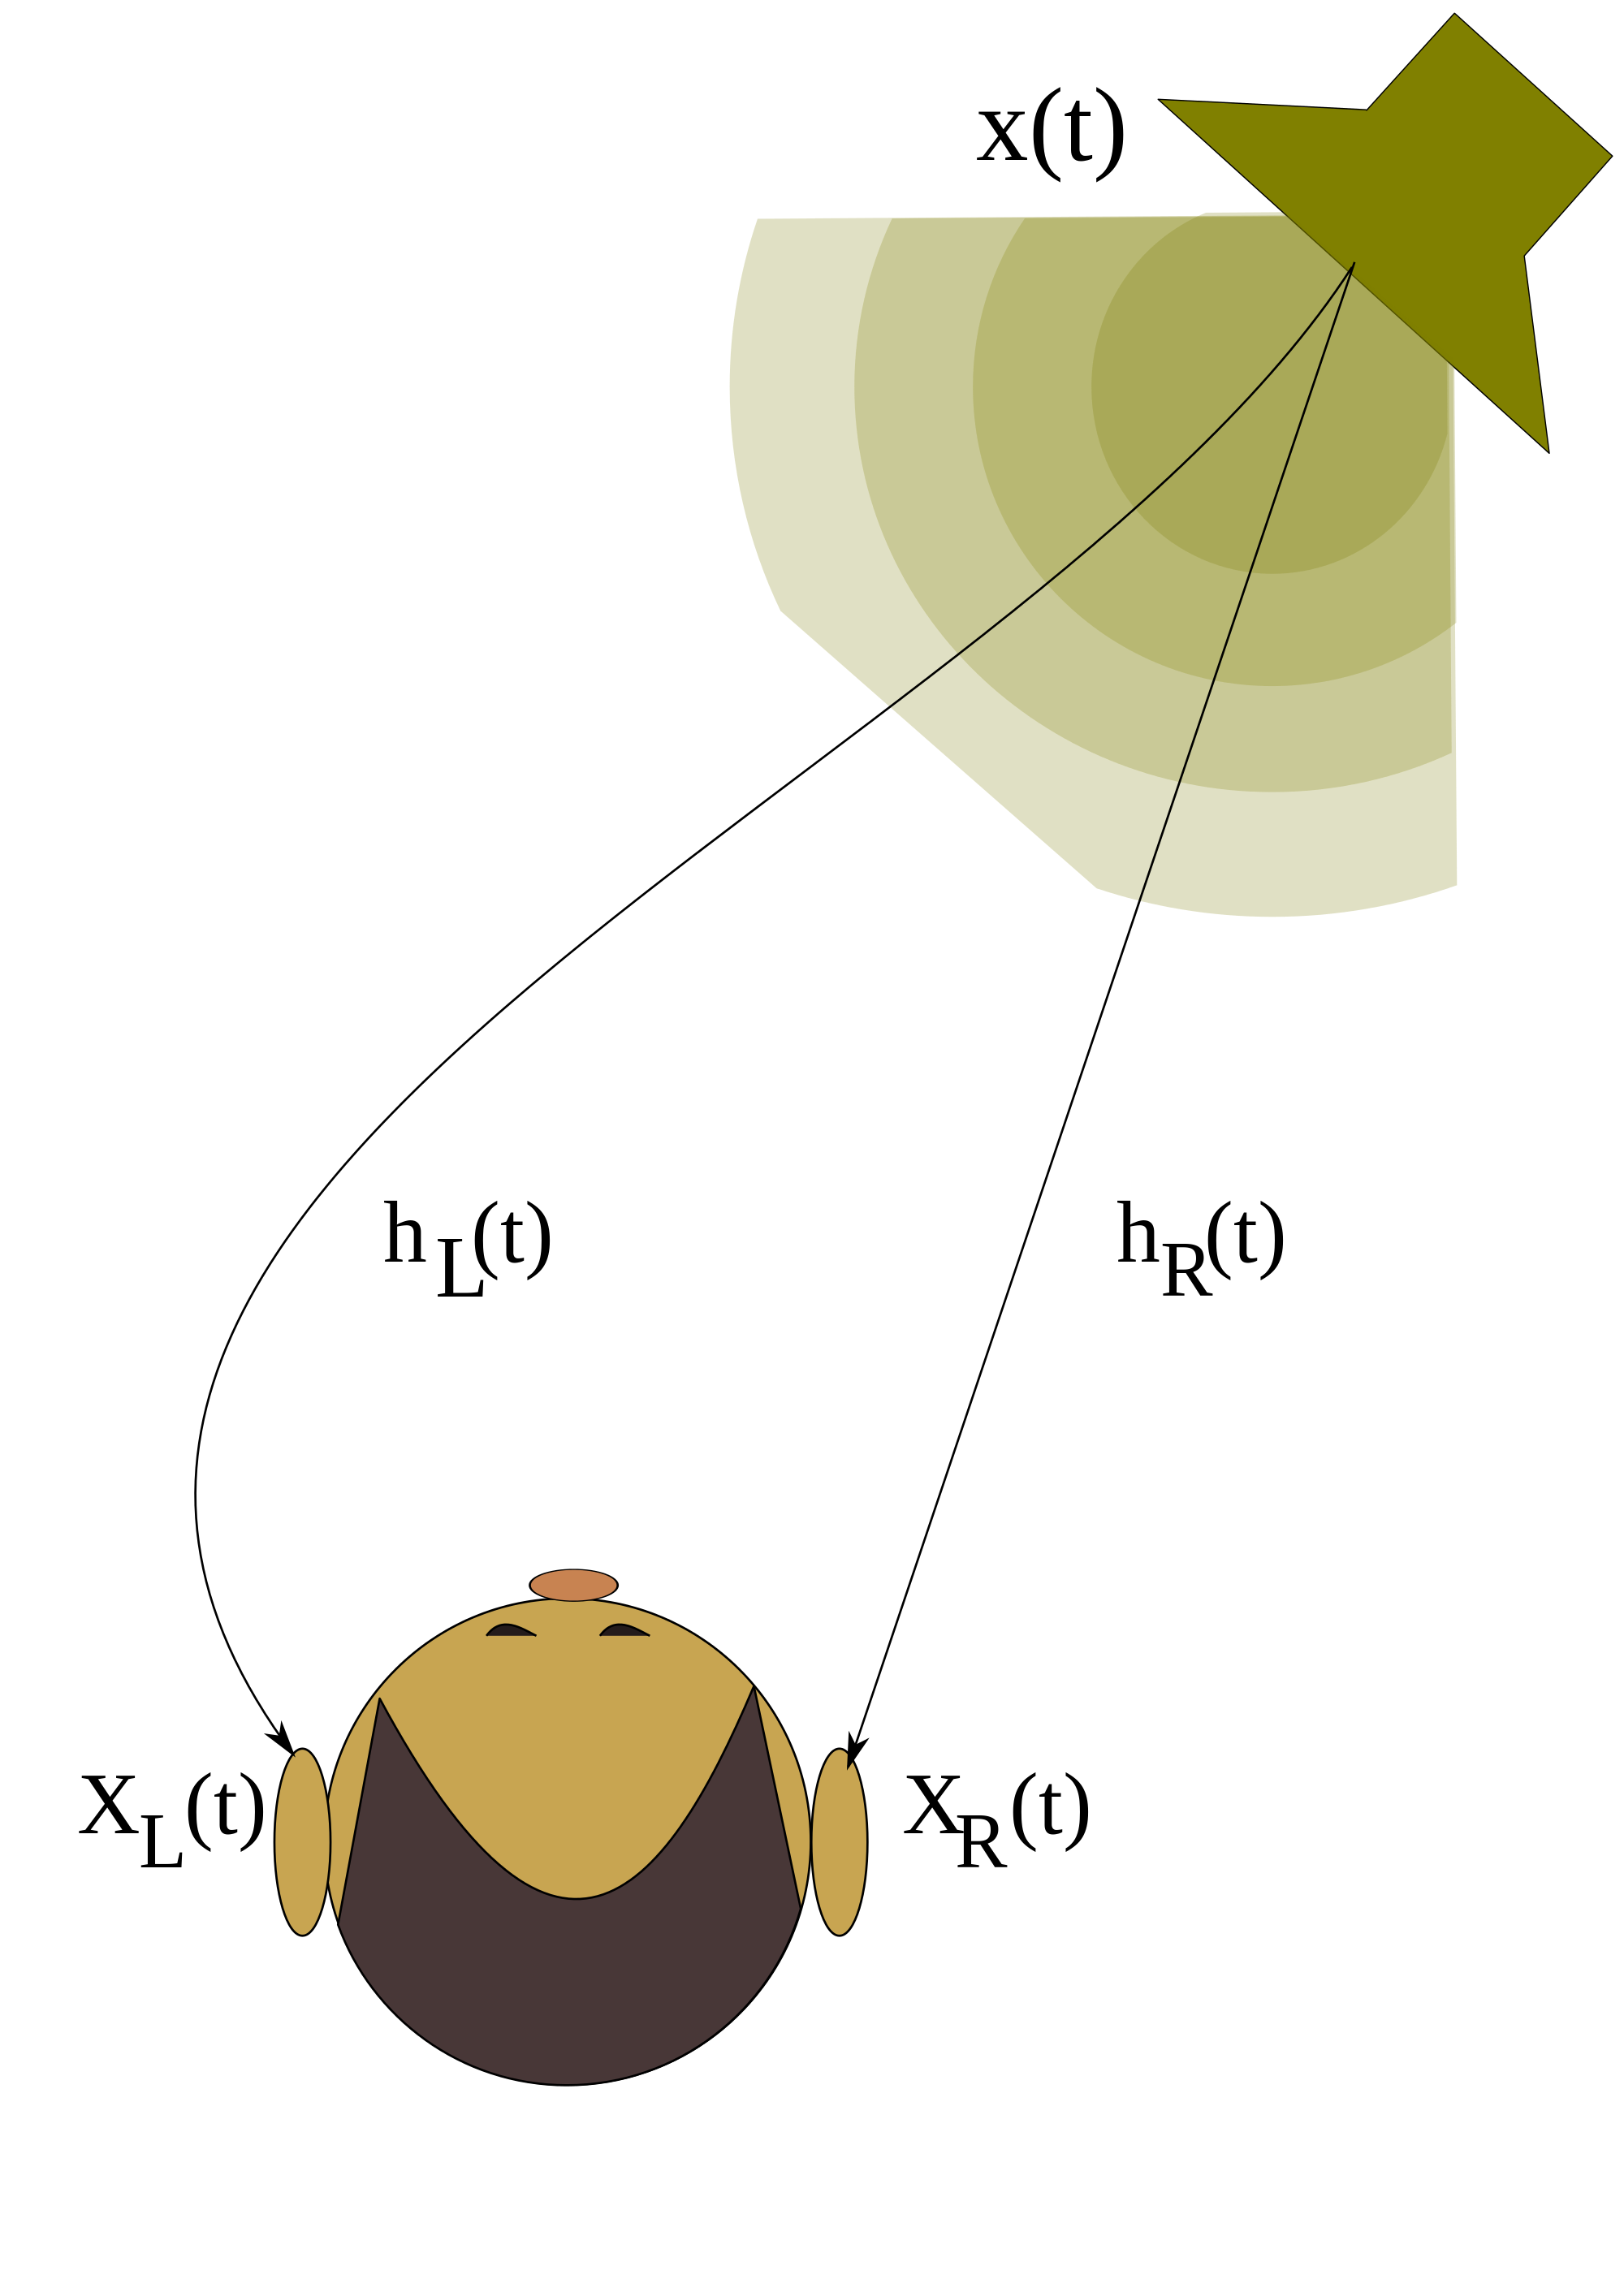
\includegraphics[scale=0.08]{hrtf.png}
    \caption{Difference in time before sounds picked up by left and right ears}
    \label{fig:idt}
\end{figure}
\end{center}

\subsection{HRTF - Head Related Transfer Function}
  
A head related transfer function describes how the sound changes as it's filtered through a listener's head. This function, or rather set of functions, describe how the sound will arrive to the listener from a specific direction. It describes how the sound is filtered based on the diffractive and reflective properties of a listener's head, pinnae and torso.\\
The measurements needed to obtain an HRTF are quite tricky and unpleasant, as they involve multiple measurements to obtain complete information about filtering from all sources.\\
There are several ways of obtaining an HRTF. One of them is to directly measure the HRIR or head related impulse response $h(t)$ at the entrance of the auditory canal (placing microphones in the tests subject's ears) as a response to an impulse $\delta(t)$ in the time domain. If the Fourier Transform $H(f)$ of $h(t)$ is taken, the desired HRTF will be obtained. This recording process is usually carried out in an anechoic chamber in order to minimize the effects early reflections and reverberations that would otherwise distort the picture. This approach is much better as the measurements need only be made once and there are already open source projects that contain multiple such measurements for multiple test subjects.\cite{cipic1}\\


The measurements we'll be using, recorded at the University of California Davis, use a special Interaural Polar Coordinate system characterized by two variables(fig \ref{fig:azel}). \cite{cipic2} $H(\theta,\phi)$:
\begin{itemize}
\item $\theta$ - azimuth or deflection of the source in the horizontal plane
\item $\phi$ - elevation or deflection in the vertical plane
\end{itemize}

\begin{center}
\begin{figure}[H]
    \centering
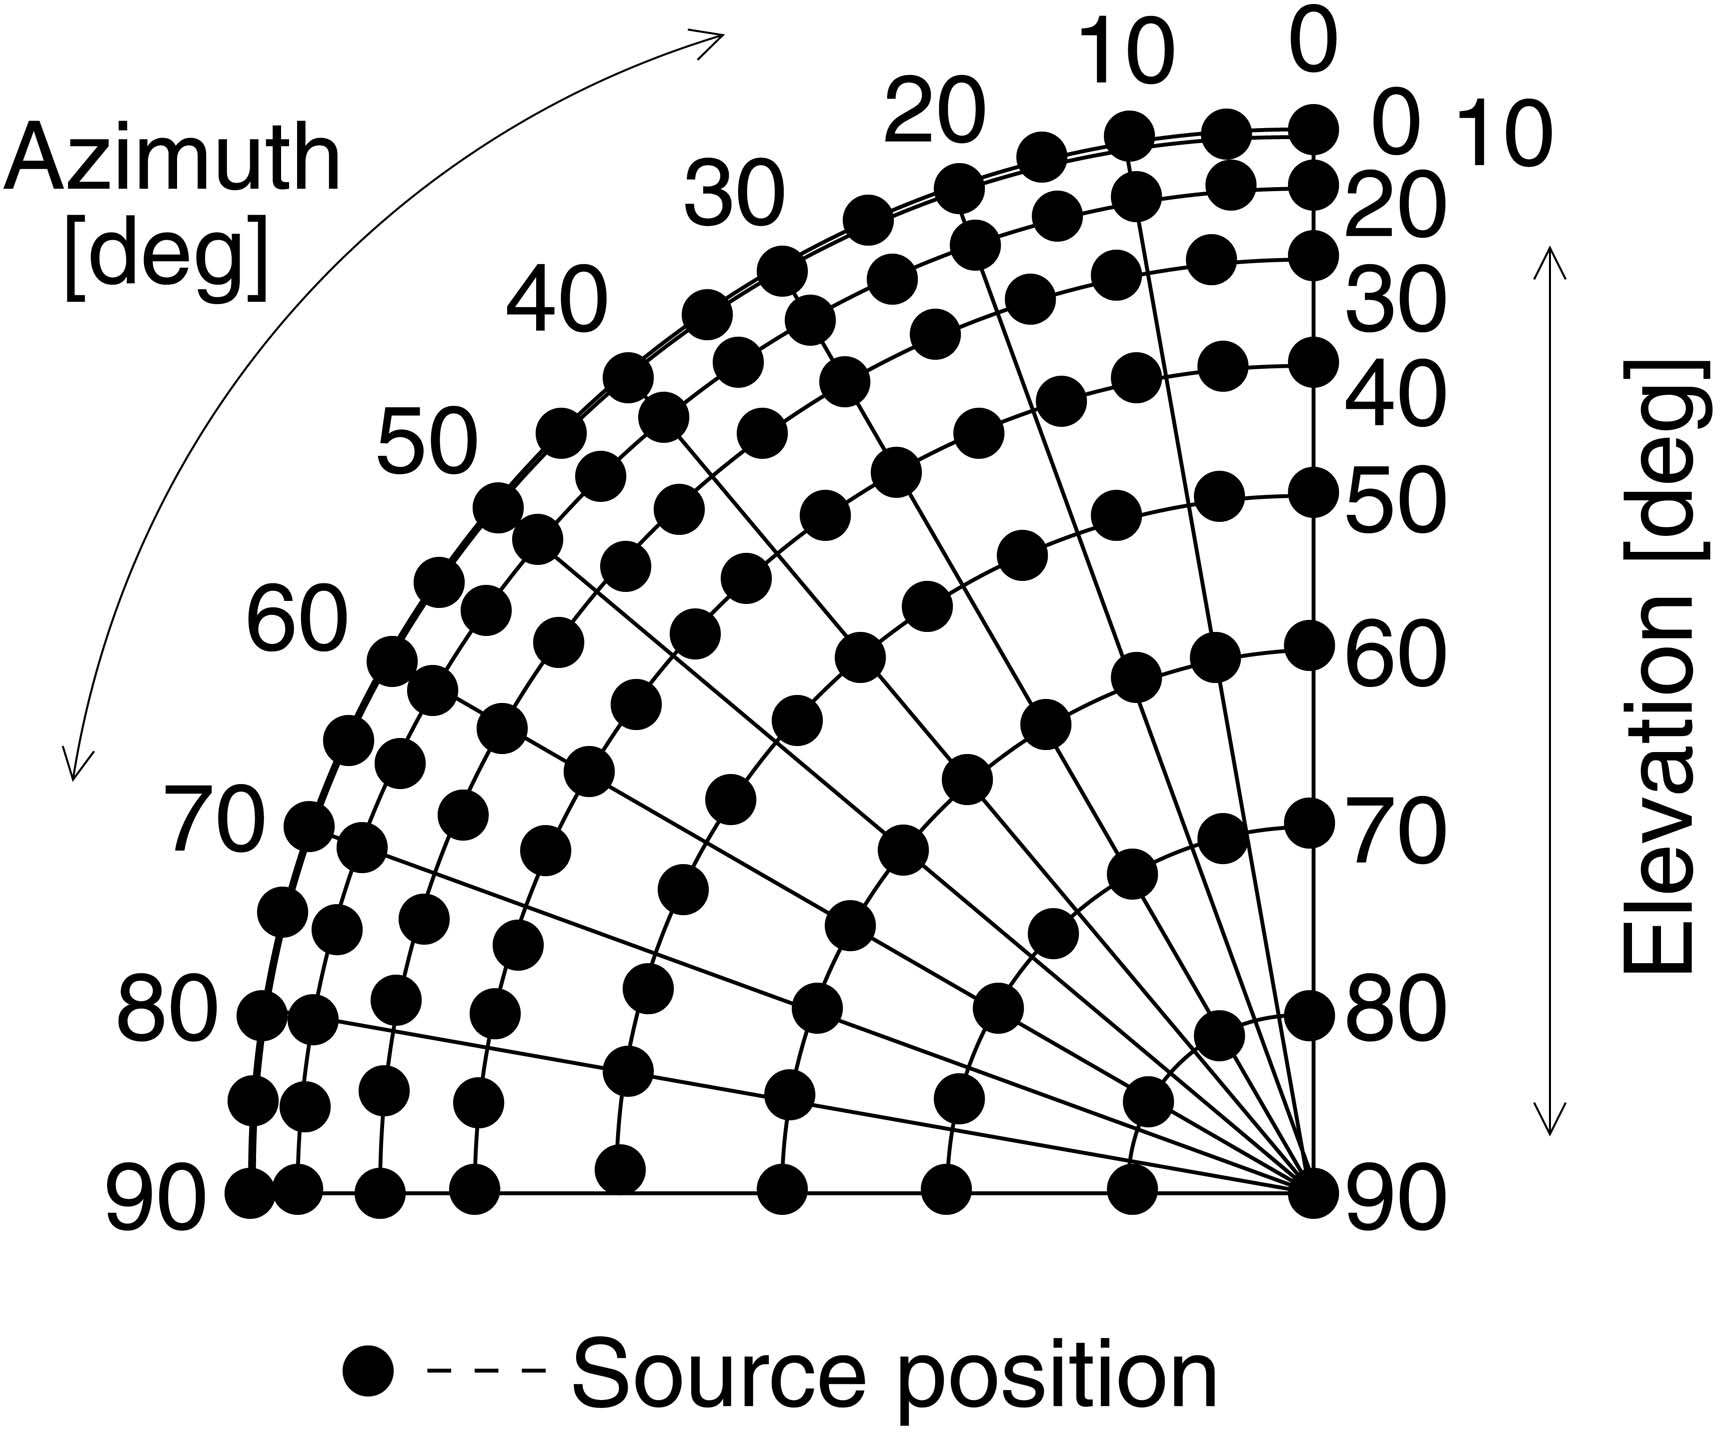
\includegraphics[scale=0.7]{src.jpg}
    \caption{Azimuth and Elevation visualized}
    \label{fig:azel}
\end{figure}
\end{center}

It is thus easy to deduce that the measurements must be carried out for multiple discrete values of these variables. (fig \ref{fig:hrtf}) Intermediate values can later be interpolated during processing. There are however some drawbacks to this method: 
\begin{itemize}
\item Requires generation of high magnitude impulse in time domain (to maximize SNR)
\item High volume impulse can be damaging to the listener's ears (especially if carried out over and over which is a must in this case)
\end{itemize}
It is thus often easier and more common to obtain the HRTF directly in the frequency domain using a frequency swept sine wave.\\
There is quite a number of systems that use HRTFs to create virtual surround sound. Many of the high end sound card have this function built in. What's novel about this particular project is the fact that head tracking is being introduced into the equation.\cite{iid1}

\begin{center}
\begin{figure}[H]
    \centering
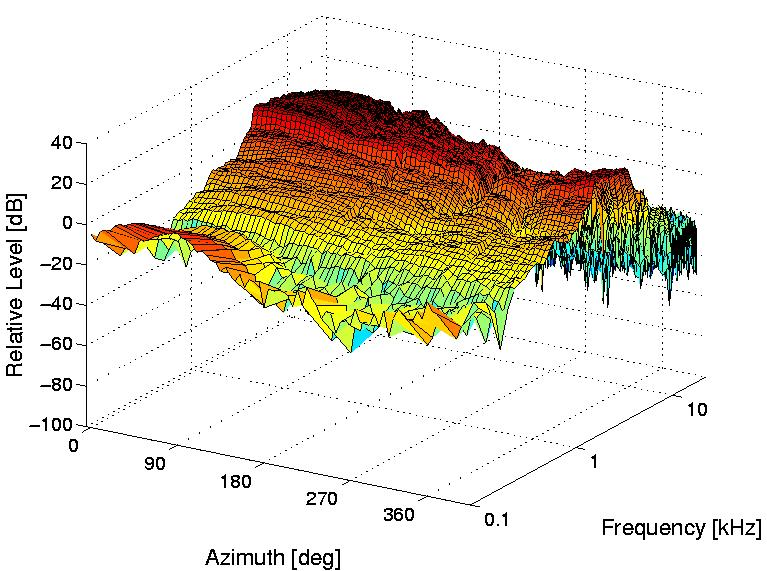
\includegraphics[scale=0.3]{hrtfsurf.jpg}    \caption{HRTF visualized with regards to Frequency and Azimuth}
    \label{fig:hrtf}
\end{figure}

\end{center}  
  
\subsection{Head Tracking}

Head Tracking is what brings this system together. If there is a way of measuring the position and orientation of a subject's head in real time, an effective means of performing real time binaural panning can be achieved. The input sound is split into multiple channels all of which are assigned to virtual positions in 3D space. The head tracker data can be used to filter the sounds such that they appear static in the global reference frame. The processing is then just a matter of doing straightforward, albeit intensive, calculations.
There's two general approaches to head tracking and both have some drawbacks associated with them. The first approach is to use head mounted sensors such as accelerometers, gyros magnetometers etc. The benefits that an approach like this brings is portability of the system as it is untethered and not restricted do a specific section of space. The listener can move around freely in any environment. This approach introduces the problem of drift due to constant round off errors during data acquisition. After a certain amount of time has passed, the measured apparent orientation will start drifting from the actual one.
Another approach is using beacons (IR emitters for instance) mounted on the head set coupled with one central unit (IR camera). This approach eliminates the problem with drift, however the user becomes confined to a closed space within the range of the IR camera and furthermore the problem of line of sight is added.\cite{rob1}\\ 
  
\section{Overview of Technologies and Hardware}

\subsection{MAX/MSP}

For the Implementation of this project Cycling74's Max 7 was chosen \cite{max}. Max is a visual programming language that was developed as a fork from the open source Pure Data language. This piece of software is highly modular with most modules or objects exist as a shared library. Max MSP deals in terms of patchers(fig \ref{fig:patc}) - a series of interconnected objects each of which serves a particular purpose and can be thought of as a black box that serves a particular task. One of the benefits of using an approach like this is the ability to get immediate feedback from the changes that are introduced to the patcher, since all of the objects have their own lifetime within the environment the moment they receive an input they start performing the necessary operations and producing output. This allowed to streamline the development cycle significantly. This approach also helps think of the problem as a conventional engineering one as it's suits an electrical engineers way of thinking. One important factor behind this choice was have the ability to abstract from infrastructural parts of the implementation and have a reliable environment for quickly accessing high quality audio from various sources. Having a working backbone made it possible to not worry about getting audio I/O to function and rather focusing on just the audio processing and headtracking parts. Since This Implementation was done on 64-bit Windows(the SDK's methods for adding the object to the DSP chain differ quite a bit between the 32- and 64-bit implementations) it was important to access external audio output devices directly, bypassing Microsoft's complicated audio pipeline. Using Max allowed for outsourcing of driver communication to an existing stable and well tested software. One of the chief reasons why using external drivers is a must is the issue of high latency and increased processor load when utilizing native Windows drivers.\\
Cycling74 also provides an extensive and well documented SDK\cite{maxsdk} for compiling custom objects to be used int patchers. The SDK is for the C programming language a language. This provides a really nice systematized framework for coding the particular behavior that is required. These objects can be compiled as dynamically linked libraries into .mxe (32-bit system) and .mxe64 (64-bit system) extensions, which if placed in Max's search path can be directly added to the patcher.\\
Cycling74 also provides a barebones runtime environment for Max which making it possible to run on any windows machine.

\subsection{Invensense MPU 6050}

To implement the headtracking part the accelerometer/gyro approach was picked. Invensense MPU 6050 was chosen for this task. Since it packs both an accelerometer and a gyroscope it has six degrees of freedom which means that it suffers less form the accumulated drift over time. Moreover it can further be daisychained with an additional magnetometer to provide even more reliable values. The sensor can be interfaced with over the serial i2c protocol. The chip also packs a special motion processor that can take care of processing of acquired data, however the manufacture does not provide a documentation on its usage to private customers. A third party open source library\cite{i2c} was used to obtain the necessary values from the raw data obtained from the sensor.\cite{mpu1} 

\subsection{Arduino} 

To Interface the MPU Arduino dev board was used. The boards were readily available in the Lab for the embedded system's course provided by prof. Hu. Arduino supports the i2c protocol. The board can be easily accessed as a I/O stream in a C program over a virtual com port and directly written to and read from. It provided a nice alternative to dedicated i2c interface as using it in custom applications is fairly easier. Arduino IDE provides the wire \cite{wire} library specifically for interfacing i2c devices. Jeff Rowberg's i2cdev library\cite{i2c} was used to talk to the MPU 6050 sensor. \cite{ard}

\section{Implementation}

The implementation of this system can roughly be broken up into two parts:
\begin{itemize}
\item Audio - the section that performs audio processing.
\item Head-tracking - the module that keeps track of user's orientation.
\item Max MSP Patcher - the patcher that ties the two sections together and provides the framework and the environment for the final result.

\end{itemize}

To fit into the time-line some of the proposed capabilities were left out, to keep the system complexity low for the purposes of this implementation. The system is tethered as incorporating Bluetooth headphone connectivity was out of scope of this project. With this limitation in mind the communications between the sensor and the software are carried out over a USB cable. The limitations on the number of input channels are limited by the performance of the system the patcher is running on. 4 channels were successfully tested. however there is no indication that significantly more can't be handled.\\ 

At this stage position tracking is also left out. A proposed solution to this problem is either using an IR camera with a couple of IR beacons, wireless ranging or ultrasonic beacons. However this is a feature that might be added In further iterations.\\

\section*{Audio}

The audio processing section consists of two parts a convolver object that convolves the input buffer with the appropriate impulse response, and an IDT object that applies the appropriate delay to the two two input channels.


\subsection{convolver Object}

Compiled as dynamically linked library convolver.mxe64 is a Max external object written in C. It has two control inlets and a signal inlet. When loaded into the Max environment it parses two .csv files (one per ear) generated in Matlab from the data provided by the CIPIC hrtf database. The impulse responses are specified for 25 azimuths (-80\degree , 80\degree ) and 50 elevations (-45\degree , 235\degree ) and 200 instances of time.\\

\begin{itemize}
\item (0\degree ,0\degree ) corresponds to a point directly ahead
\item (0\degree , 90\degree ) corresponds to a point directly overhead
\item (0\degree , 180\degree ) corresponds to a point directly behind
\item (0\degree , 270\degree ) corresponds to a point directly below
\item (90\degree , 0\degree ) corresponds to a point directly to the right
\item (-90\degree , 0\degree ) corresponds to a point directly to the left
\end{itemize}

The control inputs are supposed to be used with the format arduino\_accel\_gyro Object is outputing them, namely as indices in the array that contains the results of .csv parsing. Each time a new values is received at the control inlets the state variables defined in the struct for the object are updated and the appropriate chunk of the array is used in the convolution.\\
Since we're dealing with audio we are working with the MSP section of Max. the object has it's own lifetime. The memory for it get's allocated in the \_new() call here the object is essentially spliced into the Max dsp chain, the internal methods are bound to inlets and outlets in the main method and the object get deallocated in the \_dsp\_free() call. the processing happens in the \_perform64() high priority thread function which is in the callback method of the audio driver. Essentially once a chunk of incoming signal of a fixed vector size is received the object does the processing and writes the result to the output stream.\\
The object utilizes a fairly straightforward convolution algorithm with overlap-add for stitching the separate buffers together.\\

The convolution algorithm:


\begin{verbatim}

void convolve(t_convolver *x){

	for (int n = 0; n < OUT_SIZE; n++){

		t_double L_s, R_s;
		L_s = R_s = 0;
		size_t kmin, kmax, k;
		kmin = (n >= IN_SIZE - 1) ? n - (IN_SIZE - 1) : 0;
		kmax = (n < HRIR_SIZE - 1) ? n : HRIR_SIZE - 1;

		for (k = kmin; k <= kmax; k++){
        
			L_s += x->buff[n - k] * x->buff_h[0][k];
			R_s += x->buff[n - k] * x->buff_h[1][k];

		}
		
		if (n>=IN_SIZE){
        
			x->buff_overlap[0][n-IN_SIZE] = L_s*0.5;
			x->buff_overlap[1][n-IN_SIZE] = R_s*0.5;
		}
        
		else{
        
			x->buff_out[0][n] = L_s*0.5;
			x->buff_out[1][n] = R_s*0.5;
		}
	}
}

\end{verbatim}

The overlap-add algorithm:

\begin{verbatim}

void overlap(t_convolver *x){

	for (int i = 0; i < OUT_SIZE - IN_SIZE; i++){
    
		x->buff_out[0][i] += x->buff_overlap_prev[0][i];
		x->buff_overlap_prev[0][i] = x->buff_overlap[0][i];
		x->buff_out[1][i] += x->buff_overlap_prev[1][i];
		x->buff_overlap_prev[1][i] = x->buff_overlap[1][i];
	}
}

\end{verbatim}

The \_perform64() method:

\begin{verbatim}

void convolver_perform64(t_convolver *x, t_object *dsp64, double **ins, long numins, 
double **outs, long numouts, long sampleframes, long flags, void *userparam){

	t_double *in = ins[0];
	t_double *outL = outs[0];
	t_double *outR = outs[1];	
	int h, t;
	h = t = 0;
	int frames = sampleframes;
	
	while (sampleframes--){
    
		x->buff[h] = *in++;
		h++;
	}

	convolve(x);	
	overlap(x);

	while (frames--){
    
		*outL++ = x->buff_out[0][t];
		*outR++ = x->buff_out[1][t];
		//*outL++ = 0;
		//*outR++ = 0;
		t++;
	}	
}

\end{verbatim}

As can be seen from the snippets above the algorithm performs a fixed size convolution on the incoming signal producing two output signal from it, one intended for the left ear the other for the right.


\subsection{IDT Object}

The IDT object shares most properties with the convolver object. The difference here is that it parses the IDT values and simply delays one of the two input channels by the appropriate sample count, calculated from the sampling frequency and values obtained from the IDT.csv file.\\

The delay algorithm:

\begin{verbatim}

void IDT_perform64(t_IDT *x, t_object *dsp64, double **ins, long numins, 
double **outs, long numouts, long sampleframes, long flags, void *userparam)
{
	t_double *inL = ins[0];
	t_double *inR = ins[1];

	t_double *outL = outs[0];
	t_double *outR = outs[1];	

	
	while (sampleframes--){
		x->buff_out[0][x->h] = *inL++;
		x->buff_out[1][x->h] = *inR++;

		*outL++ = x->buff_out[0][x->tl];
		*outR++ = x->buff_out[1][x->tr];

		x->h++;
		x->h = x->h%BUFF_SIZE;

		if (x->az < 13){
			x->tl = x->h + delay_samples(x) % BUFF_SIZE;
			x->tr = x->h;
		}	
		else{
			x->tr = x->h + delay_samples(x) % BUFF_SIZE;
			x->tl = x->h;
		}
	}
}

\end{verbatim}

These two modules are incorporated into the patcher and take care of the audio processing.

\section*{Headtracking}


\subsection{Hardware}

The hardware part of this implementation is fairly straightforward. The Arduino is connected to the PC via standard USB type-B cable. The MPU 6050 is hooked up the Aduino's A4(SDA), A5(SCL), +5v(VCC), GND(Ground) pins over a 4 lead wire soldered to the breakout board. The breakout board with the sensor is attached to the headband of the AKG K401 headphones. The audio is piped to the headphones through a Focusrite 2i2 USB audio interface for high fidelity audio reproduction. The driver for this interface uses the ASIO driver allowing for low latency output.

\subsection{Arduino Sketch}

The Arduino dev board is flashed with custom firmware written in C++. The firmware initializes the sensor and configures a fifo buffer for accelerometer/gyro data processing. The sketch keeps idling until it detects a request for a new frame of values on the serial input. The data is retrieved in the form of a quaternion from the sensor and converted into Euler angle form before being written to the serial output.\\

Initializing and Configuring the Sensor:

\begin{verbatim}

void setup() {

  Wire.begin();
  TWBR = 24; // 400kHz I2C clock (200kHz if CPU is 8MHz)

  Serial.begin(115200);

  mpu.initialize();

  while (Serial.available() && Serial.read()); 

devStatus = mpu.dmpInitialize();

  // offsets for the sensor
  mpu.setXGyroOffset(220);
  mpu.setYGyroOffset(76);
  mpu.setZGyroOffset(-85);
  mpu.setZAccelOffset(1788); 
  
  if (devStatus == 0) {
    
    mpu.setDMPEnabled(true);

    attachInterrupt(0, dmpDataReady, RISING);
    mpuIntStatus = mpu.getIntStatus();

    dmpReady = true;

    packetSize = mpu.dmpGetFIFOPacketSize();
  } else {
    // ERROR!
  }
  pinMode(LED_PIN, OUTPUT);
}

\end{verbatim}

Reading the values and writing them to serial:

\begin{verbatim}

void loop() {
  digitalWrite(13, LOW);

  if (!dmpReady) return;

  mpuInterrupt = false;
  mpuIntStatus = mpu.getIntStatus();

  fifoCount = mpu.getFIFOCount();

  if ((mpuIntStatus & 0x10) || fifoCount == 1024) {
    mpu.resetFIFO();

  } 
  else if (mpuIntStatus & 0x02) {
    while (fifoCount < packetSize) fifoCount = mpu.getFIFOCount();

    mpu.getFIFOBytes(fifoBuffer, packetSize);

    fifoCount -= packetSize;

    char c = Serial.read();
    
    if(c == 'a'){
            mpu.dmpGetQuaternion(&q, fifoBuffer);
            mpu.dmpGetEuler(euler, &q);
            Serial.print(euler[0] * 180/M_PI);
            Serial.print(",");
            Serial.print(euler[1] * 180/M_PI);
            Serial.print(",");
            Serial.print(euler[2] * 180/M_PI);
            Serial.print(",");

      digitalWrite(13, HIGH);
      
    }

    blinkState = !blinkState;
    digitalWrite(LED_PIN, blinkState);
  }
}

\end{verbatim}

\subsection{arduino\_accel\_gyro Object}

The final piece is responsible for reading the values Arduino outputs and outputting them in a form that's readable by Max objects. Once instantiated the object opens a serial connection to a predefined COM port. The object has a single inlet which it uses to detect a bang (a special type of message used in the Max environment to trigger events). This inlet is used to set the timing for polling the sensor using Max's built in qmetro  (threadsafe) object. On bang detection the object writes a predefined character to the serial output and after waiting for the time it takes for arduino to write to serial, reads the new frame of values. These values are then converted into the for that is compatible with the convolver and IDT objects as specified in the CIPIC data documentation and output through the two outlets of the object.\\ In addition to that the arduino\_accel\_gyro Object takes an additional bang input for the calibration of the reference frame. when the bang is detected the current state of values is stored in the state of the object to be used as an offset for centering of future values.

\subsection{The Patcher}

The patcher is a concept closely related to the Max environment. It can be thought as a netlist that is characteristic of graphical programming languages such as LabView. The patcher is where the components discussed above fit together. It takes care of timing issues. Ties the audio processing modules to the sound source whether its an ezadc object that takes care of live audio input from a microphone or the player object that plays back audio files. The processed output is piped to the ezdac object that acts as a digital to analog converter and produces output. In addition to that a couple of control knobs are included for manual adjustment audio processing objects. The patcher also responds to midi control input because ease of work with midi is a feature of Max I was really excited about.\\
The patcher:\\

\begin{center}
\begin{figure}[H]
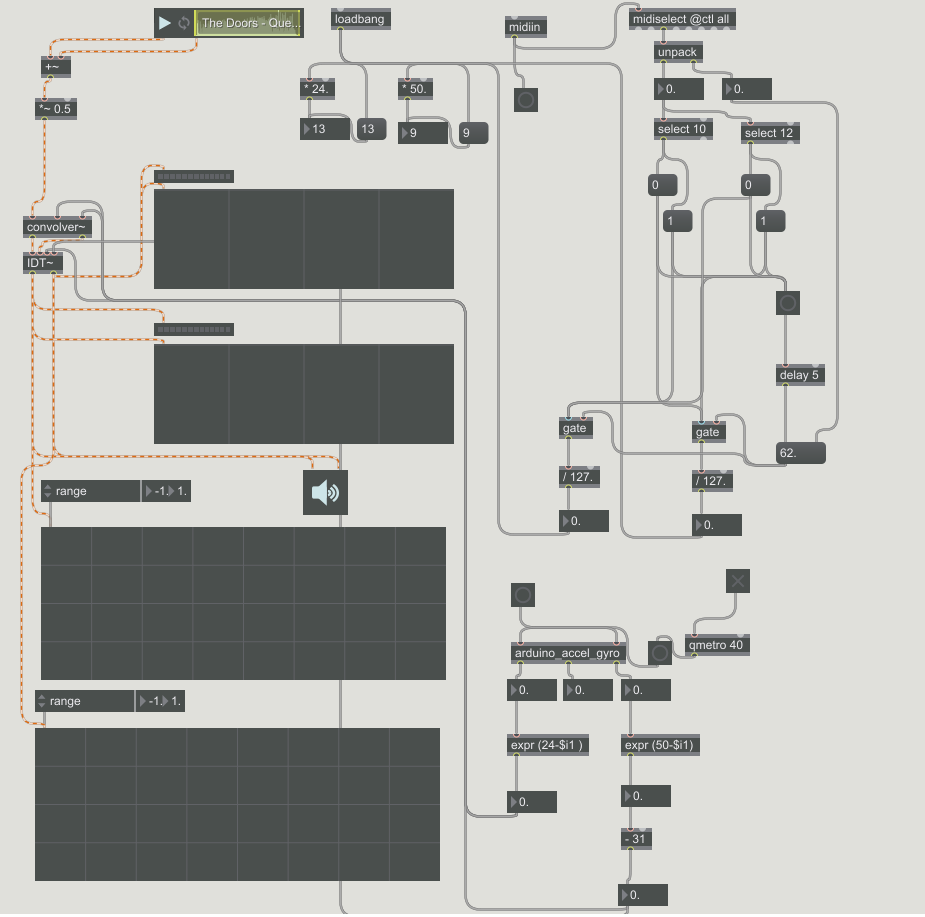
\includegraphics[scale=0.6]{patcher.png}
 \caption{Max Patching window with the project patcher}
    \label{fig:patc}
\end{figure}
\end{center}  

\section{Testing and Evaluation}

The performance of the algorithm implementation was tested against a Matlab script that simulated the buffered approach of a real time processing solution using the build in conv() method. The output produced by the patcher suffered from less auditory distortions than the Matlab script.\\

As to where the spatialization is concerned the results are harder to evaluate as the amount of directionality introduced is highly dependent on how closely the shape of the listener's head matches the head of a subject whose HRIRs were recorder. Three test were devised to asses the azimuth precision of head tracking and the ability to localize sound. The limited time and materials didn't allow for a reliable setup for measuring elevation\\

\begin{itemize}
\item Experiment One: an experiment was carried out to ascertain the head tracking properties of the system. A crude setup was created for this purpose. A circle roughly one meter in diameter was subdivided into section in appropriate angle increments. A pointer was attached to the headphones perpendicular to the plane defined by the headband to keep track of real direction. such a setup is not biased y deviations in the angle from 90\degree since the headphones were re-calibrated using the recenter button at the beginning  of the test. The values were recorded immediately after re-calibration, 5 minutes later and 15 minutes later. The Following values were obtained.

\begin {center}
\begin {itemize}

\item Average deviation over the three sets of measurements - 3.7\degree 
\item Maximum deviation over the three sets of measurements - 10\degree  (The values that are being output by accelerometer object are quantized to values with a defined response, hence values tend to be jumpy at edges between quantized regions)

\end{itemize}
\end {center}

\item Experiment Two: An experiment was carried out to test drift over time. The same setup described in the step above was used. Drift from initially calibrated center was measured after 1, 5, 15 minutes of regular intended use without pushing it to extremes.\\

\begin{center}
\begin {itemize}

\item over 15 minutes 5\degree  drift was accumulated. quantization comes into play as well here.

\end {itemize}
\end{center}

\item Experiment Three: An experiment was carried out to ascertain the precision of localization. The test was performed on 4 subjects for 3 azimuths. First the sound source was fixed in the left hemisphere and the listener was asked to look directly at where the sound appeared to come from. The process was then repeated for the right hemisphere. Finally the sound source was centered and the listener was asked to look away for 10 seconds and then look back directly at the apparent position of the sound. Here the dissimilarities between the listener's HRIR and the HRIR being used introduce a major source of error, hence a test like this is not too reliable.

\begin {center}
\begin {itemize}

\item Average deviation over the  measurements - 4.6\degree 
\item Maximum deviation over measurements - 10\degree 
\end{itemize}
\end {center}

\end{itemize}

Further notes on testing and evaluation:
\begin{itemize}
\item Head-tracking - The system is able to track the position of the listeners head with desired precision. There is a perceptible amount of drift over time, however since the patcher recenter button the system can be recalibrated at any point. Moreover the sensor has 6DoF and the data that is used is recorded with just 2DoF so head tracking precision issues don't affect it too much
\item DSP - The system is capable of performing appropriate processing on multiple channels, while keeping the latency low and quality of the sound high. The patcher manages to perform it's processing without a significant load on the processor. The latency is imperceptible for all intents and purposes. The audio suffers from few auditory distortions when switching from one HRIR to another however this can be helped using a simple averaging filter on a frame of several samples whenever control inputs change
\item Sound - The test subjects reported that the effect introduced was "clearly distinguishable" and introduced "imperceptible" to "unobtrusive" auditory artifacts (mostly in form of low volume clicks mentioned above)
\item The listeners recorded jumps between sides if the setup is turned to extremes. This is unavoidable since the azimuths are defined in the (-80, 80) and there is bound to be a jump after a 180\degree rotation in either directions.
\end{itemize}

\section{Deliverable}

The final result of this project is a Max patcher, that utilizes Max externals coded up for this purpose specifically. The patcher keeps track of the user's head orientation and processes the audio appropriately. The software part has to be coupled with an Arduino equipped with a accelerometer/gyro senser mounted on the listener's head. The patcher can be run on a 64-bit windows machine (both in standalone Max and in the Max runtime) since the externals' compilation setting target this particular platform and the API calls for the 64-bit version are used.

\section{Conclusions}

The implementation presented in the sections above does the core task of tracking the user's head and processing the audio respectively. There are several proposed features that could not be implemented due to time constraints and unavailability of particular hardware such as untethered's implementation, position tracking etc... However the core is there, moreover since it's mostly written in C it can serve as a blueprint for a native C app provided the audio section is taken care of.  
    
  \newpage
  
  \bibliographystyle{unsrt}
  \bibliography{bibliography}
  
  

\end{document}
